\documentclass[border=10pt]{standalone}
\usepackage[svgnames]{xcolor}
\usepackage{amsmath}
\usepackage{pgfplots}
\pgfplotsset{compat=newest}
\usepackage[sfdefault]{FiraSans}
\usepackage{FiraMono}
\renewcommand*\familydefault{\sfdefault}
\begin{document}
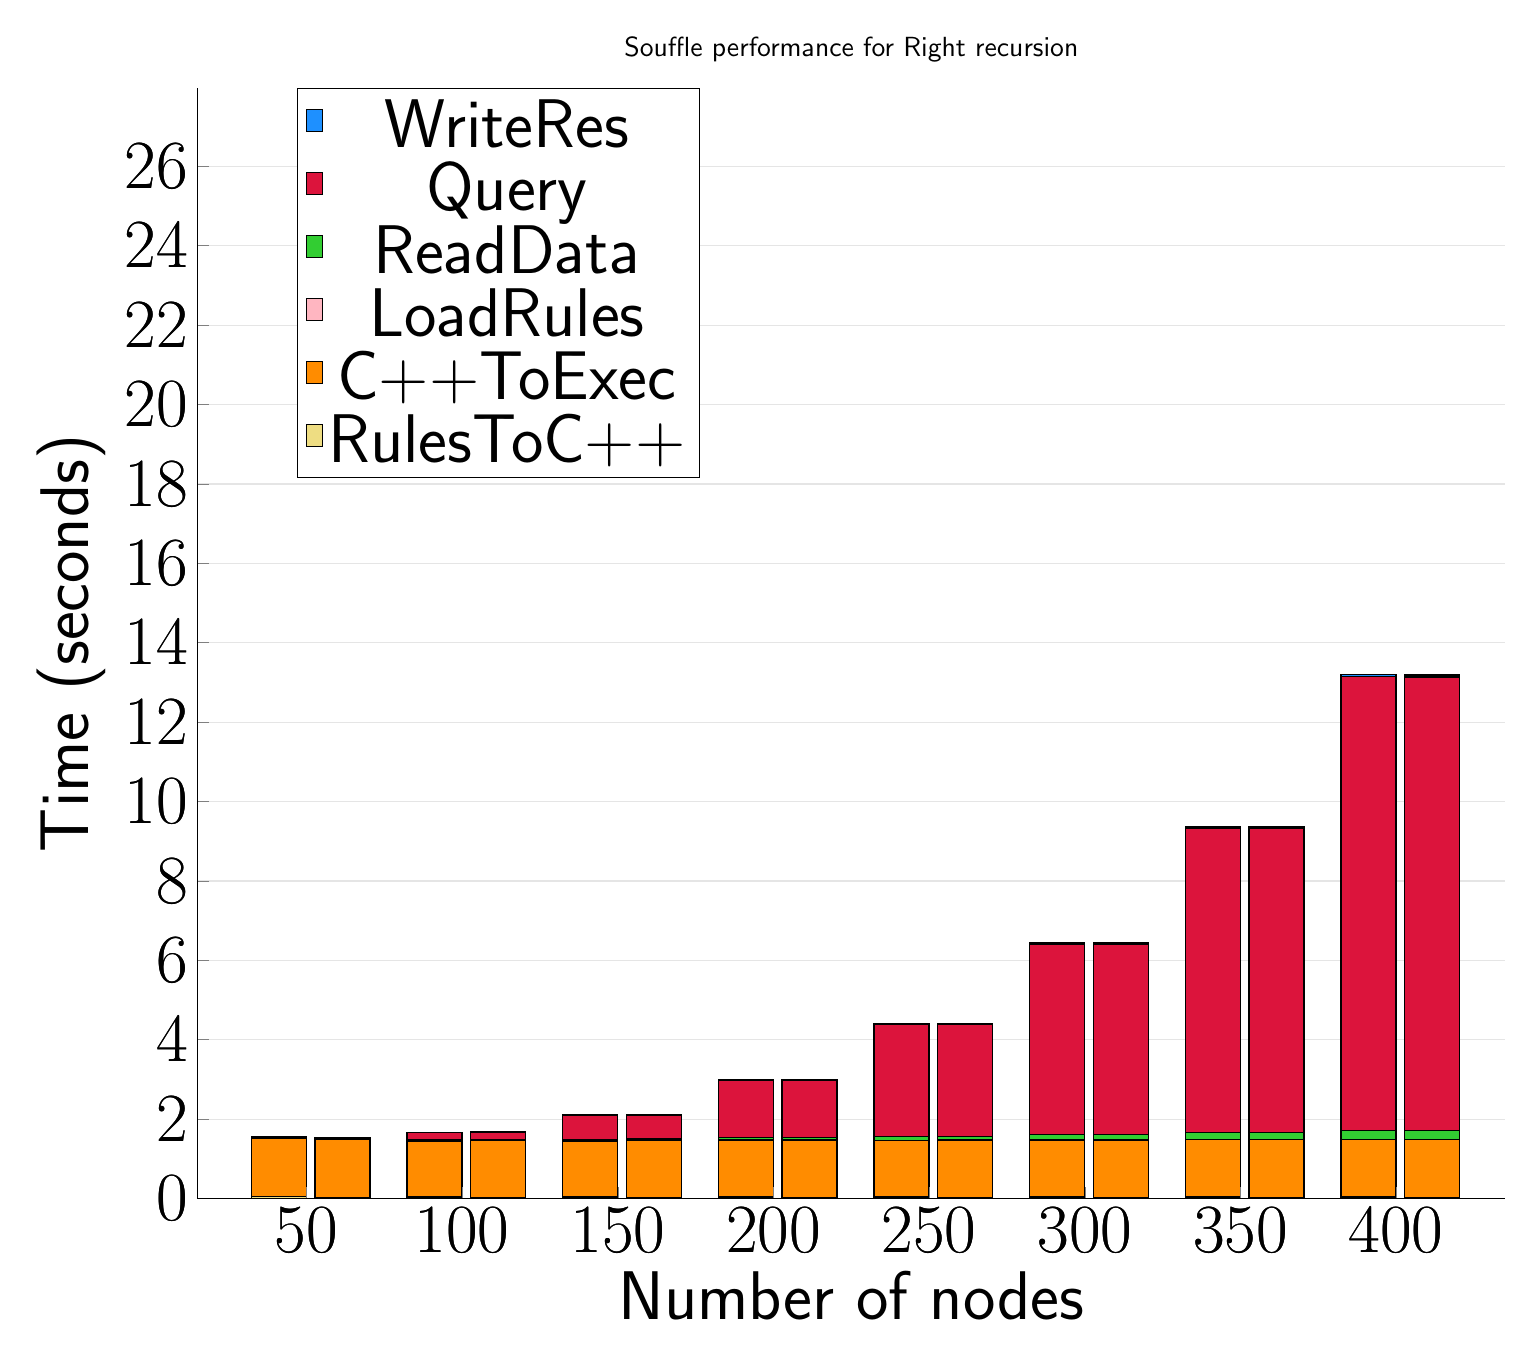
\begin{tikzpicture}
	\begin{axis}[
			ybar stacked,
			title={Souffle performance for Right recursion},
			bar shift=-10pt,
			width=1.5\textwidth,
			bar width=0.7cm,
			ymajorgrids, tick align=inside,
			major grid style={draw=gray!20},
			xtick=data,
			ymin=0, ymax=27.977500000000003,
			axis x line*=bottom,
			axis y line*=left,
			enlarge x limits=0.1,
			legend style={
					at={(0.23, 1)},
					anchor=north,
					legend columns=1,
					font=\Huge,
				},
			ylabel={Time (seconds)},
			xlabel={Number of nodes},
			label style={font=\Huge},
			tick label style={font=\Huge},
		]
		\addlegendimage{fill=DodgerBlue, draw=black, line width=0.2pt}
		\addlegendentry{WriteRes}
		\addlegendimage{fill=Crimson, draw=black, line width=0.2pt}
		\addlegendentry{Query}
		\addlegendimage{fill=LimeGreen, draw=black, line width=0.2pt}
		\addlegendentry{ReadData}
		\addlegendimage{fill=LightPink, draw=black, line width=0.2pt}
		\addlegendentry{LoadRules}
		\addlegendimage{fill=DarkOrange, draw=black, line width=0.2pt}
		\addlegendentry{C++ToExec}
		\addlegendimage{fill=LightGoldenrod, draw=black, line width=0.2pt}
		\addlegendentry{RulesToC++}
		\addplot +[fill=LightGoldenrod, draw=black, line width=0.5pt] coordinates {
				(50, 0.05000002384185791)
				(100, 0.03900001049041748)
				(150, 0.040000200271606445)
				(200, 0.040999984741210936)
				(250, 0.04000000953674317)
				(300, 0.04000000953674317)
				(350, 0.04000003337860107)
				(400, 0.041999983787536624)
			};
		\addplot +[fill=DarkOrange, draw=black, line width=0.5pt] coordinates {
				(50, 1.474999976158142)
				(100, 1.4129999876022339)
				(150, 1.4119998455047607)
				(200, 1.430999994277954)
				(250, 1.4239999771118164)
				(300, 1.4320000410079956)
				(350, 1.446999979019165)
				(400, 1.440999984741211)
			};
		\addplot +[fill=LightPink, draw=black, line width=0.5pt] coordinates {
				(50, 1.12708e-05)
				(100, 1.01917e-05)
				(150, 1.0375e-05)
				(200, 0.0)
				(250, 0.0)
				(300, 0.0)
				(350, 1.01166e-05)
				(400, 0.0)
			};
		\addplot +[fill=LimeGreen, draw=black, line width=0.5pt] coordinates {
				(50, 0.005444488000000001)
				(100, 0.020333109999999998)
				(150, 0.04114932)
				(200, 0.06530533000000001)
				(250, 0.09613055000000001)
				(300, 0.13513899999999998)
				(350, 0.1803433)
				(400, 0.2374966)
			};
		\addplot +[fill=Crimson, draw=black, line width=0.5pt] coordinates {
				(50, 0.03230454)
				(100, 0.1887831)
				(150, 0.6045111000000001)
				(200, 1.4459170000000001)
				(250, 2.818618)
				(300, 4.8076870000000005)
				(350, 7.669522000000001)
				(400, 11.43623)
			};
		\addplot +[fill=DodgerBlue, draw=black, line width=0.5pt] coordinates {
				(50, 0.0011189866)
				(100, 0.0028790119999999994)
				(150, 0.006370567000000001)
				(200, 0.011119340000000002)
				(250, 0.01740241)
				(300, 0.02512589)
				(350, 0.03408087)
				(400, 0.04499426)
			};
	\end{axis}
	\begin{axis}[
			ybar stacked,
			bar shift=13pt,
			width=1.5\textwidth,
			bar width=0.7cm,
			ymajorgrids, tick align=inside,
			major grid style={draw=none},
			xtick=data,
			ymin=0, ymax=27.977500000000003,
			axis x line*=none,
			axis y line*=none,
			enlarge x limits=0.1,
			label style={font=\Huge},
			tick label style={font=\Huge},
		]
		\addplot +[fill=LightGoldenrod, draw=black, line width=0.5pt] coordinates {
				(50, 0.031000000000000007)
				(100, 0.030000000000000006)
				(150, 0.030000000000000006)
				(200, 0.030000000000000006)
				(250, 0.030000000000000006)
				(300, 0.030000000000000006)
				(350, 0.030000000000000006)
				(400, 0.030000000000000006)
			};
		\addplot +[fill=DarkOrange, draw=black, line width=0.5pt] coordinates {
				(50, 1.4649999999999999)
				(100, 1.4369999999999998)
				(150, 1.4329999999999998)
				(200, 1.4469999999999998)
				(250, 1.4439999999999997)
				(300, 1.4439999999999995)
				(350, 1.453)
				(400, 1.454)
			};
		\addplot +[fill=LightPink, draw=black, line width=0.5pt] coordinates {
				(50, 1.11e-05)
				(100, 1.02e-05)
				(150, 1.02e-05)
				(200, 0.0)
				(250, 0.0)
				(300, 0.0)
				(350, 0.0)
				(400, 0.0)
			};
		\addplot +[fill=LimeGreen, draw=black, line width=0.5pt] coordinates {
				(50, 0.005443600000000001)
				(100, 0.0203258)
				(150, 0.0410564)
				(200, 0.0647587)
				(250, 0.09538469999999999)
				(300, 0.13409449999999998)
				(350, 0.1778328)
				(400, 0.23472890000000005)
			};
		\addplot +[fill=Crimson, draw=black, line width=0.5pt] coordinates {
				(50, 0.0322895)
				(100, 0.1887387)
				(150, 0.6043478)
				(200, 1.4434140000000002)
				(250, 2.814502)
				(300, 4.803262)
				(350, 7.660176999999999)
				(400, 11.42133)
			};
		\addplot +[fill=DodgerBlue, draw=black, line width=0.5pt] coordinates {
				(50, 0.0009866999999999999)
				(100, 0.0028780000000000003)
				(150, 0.0062959)
				(200, 0.0110188)
				(250, 0.017276600000000003)
				(300, 0.0247944)
				(350, 0.0337603)
				(400, 0.04420929999999999)
			};
	\end{axis}
\end{tikzpicture}

\end{document}
